\documentclass[10pt]{beamer}
\usepackage{amsmath}
\usepackage{amsthm}
\usepackage{tikz}
\usepackage{booktabs}
\usetikzlibrary{shapes.geometric, arrows}
\usepackage{listings}


%\usepackage{minted}


\newcommand{\R}{\mathbb{R}}
\newcommand{\C}{\mathcal{C}}
\renewcommand{\u}{\mathbf{u}}
\renewcommand{\v}{\mathbf{v}}
\newcommand{\w}{\mathbf{w}}
\newcommand{\x}{\mathbf{x}}
\newcommand{\y}{\mathbf{y}}
\renewcommand{\b}{\mathbf{b}}
\newcommand{\e}{\mathbf{e}}
\newcommand{\s}{\mathbf{s}}


\newcommand{\A}{\mathbf{A}}
\newcommand{\B}{\mathbf{B}}
\newcommand{\W}{\mathbf{W}}

%\newtheorem{theorem}{Theorem}[section]
%\newtheorem{proposition}[theorem]{Proposition}
%\newtheorem{lemma}[theorem]{Lemma}
%\newtheorem{corollary}[theorem]{Corollary}
%
%
%\theoremstyle{definition}
%\newtheorem{definition}[theorem]{Definition}
%\newtheorem{example}[theorem]{Example}


\begin{document}
\title{Recurrent Neural Networks}
\author{Jean-Martin Albert}
\date{\today}
\maketitle





\begin{frame}{A Bird's Eye View Of Classical Neural Networks}
Let $f:\R^n\to \R^m$ be a function, and consider a class $\C$ of functions $g: \R^n\to \R^m$, which we assume to be parametrized by $\R^\ell$, in the sense that there is a function $F(\x,\w):\R^n\times \R^\ell\to\R^n$ such that $\C=\{\x\mapsto F(\x,\w):\w\in\R^n\}$.  The generic problem of machine learning is to find a vector $\w\in\R^{\ell}$ such that $\ell(\w) = D(f(\x), F(\x, \w))$ is as small as possible, where $D$ represents a notion of distance between functions.
 Given the definition of $D$, we see that $\ell(\x)\geq 0$, and therefore $\ell$ has a global minimum (which is not necessarily unique). In general, the global minimum of $\ell$ is not attained, in the sense that if $\epsilon=\min\{\ell(\w):\x\in\R^n\}$, then there does not necessarily exist a value $\w_0\in\R^\ell$ such that $\epsilon=\ell(\w_0)$.  However, it can be approximated, that is to say there is a sequence $\w_i$ such that $\ell(\w_i)\to\epsilon$ as $i\to\infty$.
\end{frame}

\begin{frame}{A Bird's Eye View Of Classical Neural Networks}
In tensorflow, the function we are trying to approximate is given in the form of a relation $f(\x)=\y$. We provide {\em placeholders} for the values of $\x$ and $\y$.  The function $F(\x,\w)$ is defined by a computation graph.  For example, here is a linear regression, in which we try to approximate a function $f:\R^{10}\to\R^{15}$ using a function of the form $F(\x, \W\b)=\W\x+\b$. Here $\W$ is an $15\times 10$ matrix, and $\b\in\R^{15}$
\end{frame}

\defverbatim[colored]\lstI{
\begin{lstlisting}[language=Python,basicstyle=\ttfamily,keywordstyle=\color{red}]
x = tf.placeholder(shape=[None, 10])
y = tf.placeholder(shape=[None, 15])
W = tf.Variable(shape=[None, 10, 15])
b = tf.Variable(shape=[None, 15])
F = tf.matmul(x, W) + b
loss = tf.mean_square_error(y, F)
\end{lstlisting}
}
\begin{frame}{A Bird's Eye View Of Classical Neural Networks}
\lstI
\end{frame}






\begin{frame}{Sequences}
Classical neural networks are great for classification problems involving either fixed (finite) sets $f:A\to B$, where $A$ represents the set to be classified, and $B$ is the set of labels, or functions $f:\R^n\to B$. An example of the latter is image classification, since an $n\times m$ image can be directly represented as a vector in $\R^{\ell mn}$. In many cases, however, the data to be classified is better represented as a (finite) sequence.  For example, sentences are sequences of words, words are sequences of letters, movies are sequences of images, and sound files are sequences of amplitudes.  It is possible to deal with sequences with ordinary neural networks, but we run into difficulties when we try to model dependency between different elements of a sequence.
\end{frame}

\begin{frame}{Sequences}
Let $A$ be a finite set. A finite sequence of elements of $A$ is a tuple $(a_1,...,a_n)$, where $a_i\in A$ for every $i$.  Here the number $n$ is allowed to change.  The set of all finite sequences of elements of $A$ is denoted $A^*$.  From the definition we just gave, we have $A^*=\bigcup_{n\geq 0} A^n$, which is a good enough definition for our purpose.  If we are given two finite sets $A$ and $B$, there are many situations we can consider if we also have access to $A^*$ and $B^*$.
\end{frame}

\begin{frame}{Sequences}
  \begin{enumerate}
    \item A function $f:A\to B^*$, which given an element of $A$ outputs a sequence of elements of $B$.  This is called a {\em one-to-many} function. We use this architecture in a sequence sorting neural network. The Tweet2Vec autoencoder also uses a one-to-many neural network.
    \item A function $f:A^*\to B$, which is given a sequence of elments of $A$ and produces a single element of $B$.  This is called a {\em many-to-one} function.  A good example of sich a function is the Buzzometer sentiment analysis tool which assigns a single sentiment value to messages which can vary in length.
    \item A function $f:A^*\to B^*$ which is given a seuqence of elements of $A$< and outputs a sequence of elements of $B$.  This is called a {\em many-to-many} function.  As an example of such a function we will show the implementation of a simple text generator.  Translation, video captioning, part-of-speech tagging and speech recognition are all examples of many-to-many functions.
  \end{enumerate}
\end{frame}


\begin{frame}{Functions on Sequences}
We can of course define functions $A\to B^*$, $A^*\to B$ and $A^*\to B^*$ directly (they are just sets, after all), but it is more interesting and instructive to make use of the structure of $A^*$ and $B^*$ as sets of sequences of $A$ and $B$, and see how one can use a function (or class of functions) $A\to B$ to define a function $A^*\to B^*$. In particular, we will me making use of the iterative nature of the construction $A^*$ and $B^*$. Here is the simplest example: if $A=B$, and $f:A\to A$ is a function, then we can iterate $f$: $f^0(a)=a$ for every $a\in A$, and $f^{n+1}(a) = f(f^n(a))$. We terminate the iteration at the first value of $n$ for which $f^n(a)=f^{n-1}(a)$ (note that there is no guarantee that this will ever happen). This gives a function $f:A\to A^\omega$.
\end{frame}

\begin{frame}{Functions on Sequences}
We describe a more general situation. Let $S$ be a (finite) set of {\em states} with a distinguished element $\perp\in S$, and consider a function $f:A\times S\to B\times S$. Let $a_1,...,a_n$ be a finite sequence of elements of $A$.  We define two sequences $b_1,...,b_n$ and $s_1,...,s_n$ of elements of $B$ and $S$ respectively as follows.  We first define $b_1, s_1 = f(a_1, \perp)$.  Suppose that we have defined the elements $b_1,...,b_n$ and $s_1,...,s_n$.  We define $b_{n+1}$ and $s_{n+1}$ via $b_{n+1}, s_{n+1} = f(a_{n+1}, s_n)$.  We define $f^*(a_1...a_n)=b_1...b_n$, with $b_1,...,b_n$ defined as above.  This is a function $f^*:A^*\to B^*$, and it has the property that the length of the output sequence is the same as that of the input sequence.  An interesting special case of this is when $S=B$. In this case, we can have $f:A\times B\to B$. We can define $b_1 = f(a_1, \perp)$, and $b_{n+1}=f(a_{n+1}, b_n)$. This is in fact the main type of function we use in our examples later. Note that this is a state machine, close to a deterministic finite automaton, except that here the state space $S$ is allowed to be infinite.
\end{frame}

\begin{frame}{Functions on Sequences}
We use the exact same method to define a many-to-one function. If $f:A\times S\to B\times S$ is a function, and  $a_1,...,a_n$, $b_1,...,b_n$ and $s_1,...,s_n$ are defined as above, then we define $f^*(a_1,...,a_n)=b_n$.  In other words, we discard all elements of $B$ produced during the iteration, and keep only the last one.
\end{frame}

\begin{frame}{Functions on Sequences}
Finally, we tackle the case of a one-to-many function. Again we let $f:A\times S\to B\times S$ be any function. We define sequences $b_1,...,b_i,...$ and $s_1,...,s_i,...$ as follows. $b_1,s_1=f(a,\perp)$, and for every $n$, $b_{n+1}, s_{n+1}=f(a, s_n)$. In other words, we keep iterating $f$, feeding $a$ as input at every step. An imoprtant variant of this is when $a$ itself has a distinguished element $\perp_A$, in which case, after feeding $a$ as an input to $f$ in the first iteration, we subsequently feed it $\perp_A$, and get $b_{n+1}, s_{n+1}=f(\perp_A, s_n)$.  We stop the iteration whenever $s_n=\perp$ (or any other predetermined element of $S$). Note that this may never happen, i.e. the sequence $b_n$ may go on forever. In fact, there is no way to give a general pattern of definition for $f:A\times S\to B\times S$ which will guarantee that $f^*(a)$ is finite for every $a$.
\end{frame}

\begin{frame}{Recurrent Neural Networks}
  In general, a recurrent neural network is just a presceiption for a class of functions of the form $f:\R^n\times \R^\ell\times\R^m\to \R^m\times \R^\ell$, where $\R^m$ is the space of parameters. The set $\{0,1\}^*$ of all finite sequences of $0$'s and $1$'s is countable, and $\R^\ell$, being a real vector space,
  is uncountable.  Therefore, we can encode every element $w\in\{0,1\}^*$ as a vector in $S$.  Informally,
  $\R^\ell$ is enough to encode any finite state space, and every possible value for the content of the tape of a
  Turing machine. We get:

  \begin{theorem}
  Recurrent neural networks are Turing-complete.
  \end{theorem}

  This explains why recurrent neural networks seem to be able to produce results that other networks can't. Training a recurrent network is the same as producing a Turing machine.  A common way to represent a recurrent node is to use a box, the inside of which represent the definition of $f$.  The vertical arrows represent the input and onput of the node, and the horisontal arrows represent the input and output state of the node.
\end{frame}

\begin{frame}{Recurrent Neural Networks}
  \begin{center}
    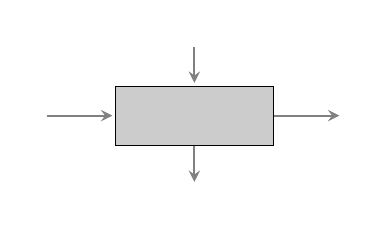
\begin{tikzpicture}[shorten >=1pt,->,draw=black!50, node distance=1cm]
      \tikzstyle{arrow} = [thick,->,>=stealth]
      \tikzstyle{startstop} = [rectangle, minimum width=2cm, minimum height=.75cm, text centered, draw=black, fill=black!20]
      \node (input) [] at (0cm,1cm) {};
      \node (output) [] at (0cm,-1cm) {};
      \node (s-input) [] at (-2cm,0cm) {};
      \node (s-output) [] at (2cm,0cm) {};
      \path[] node[startstop] (N) at (0cm,0cm) {};
      \draw [arrow] (input) -- (N);
      \draw [arrow] (s-input) -- (N);
      \draw [arrow] (N) -- (output);
      \draw [arrow] (N) -- (s-output);
  \end{tikzpicture}
  \end{center}
\end{frame}

\begin{frame}{Recurrent Neural Networks}
  ust like any regular neural network layer, recurrent nodes can be composed.  The composition of two recurrent nodes is done by feeding the output of one node into the input of the other, and concatenating their state space.  Formally, if $f:\R^n\times \R^\ell\times\to \R^m\times \R^\ell$ and $g:\R^n\times \R^\ell\times\to \R^m\times \R^\ell$ are two recurrent nodes, then we have the node $(f;g):\R^m\times\R^\ell\times\R^L\to\R^k\times\R^\ell\times\R^L$ defined by $(f;g)(\x, \s_1, \s_2) = (\y, \s'_1, \s'_2)$ where $f(\x, \s_1) = \x', \s'_1$ and $g(\x', \s_2) = \y, \s'_2$. Graphically, we can represent this by stacking the boxes representing $f$ and $g$ on top of one another:

  \begin{center}
  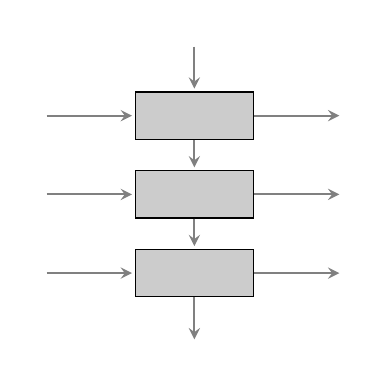
\begin{tikzpicture}[shorten >=1pt,->,draw=black!50, node distance=1cm]
      \tikzstyle{arrow} = [thick,->,>=stealth]
      \tikzstyle{startstop} = [rectangle, minimum width=1.5cm, minimum height=.6cm, text centered, draw=black, fill=black!20]
      \node (input) [] at (0cm,1cm) {};
      \node (output) [] at (0cm,-3cm) {};
      \node (s-input-A) [] at (-2cm,0cm) {};
      \node (s-output-A) [] at (2cm,0cm) {};
      \node (s-input-B) [] at (-2cm,-1cm) {};
      \node (s-output-B) [] at (2cm,-1cm) {};
      \node (s-input-C) [] at (-2cm,-2cm) {};
      \node (s-output-C) [] at (2cm,-2cm) {};
      \path[] node[startstop] (A) at (0cm,0cm) {};
      \path[] node[startstop] (B) at (0cm,-1cm) {};
      \path[] node[startstop] (C) at (0cm,-2cm) {};
      \draw [arrow] (input) -- (A);
      \draw [arrow] (s-input-A) -- (A);
      \draw [arrow] (s-input-B) -- (B);
      \draw [arrow] (s-input-C) -- (C);
      \draw [arrow] (A) -- (s-output-A);
      \draw [arrow] (B) -- (s-output-B);
      \draw [arrow] (C) -- (s-output-C);
      \draw [arrow] (A) -- (B);
      \draw [arrow] (B) -- (C);
      \draw [arrow] (C) -- (output);
  \end{tikzpicture}
  \end{center}
\end{frame}

\begin{frame}{Training RNN's}
  How do we train recurrent neural networks? we can use back propagation, just like a regular neural network. Heuristically, we unroll the recurrent network ``infinitely'' many times, until it looks like an ordinary very deep neural network.  In practice, since computers only have a finite amount of resources, we only unroll the network a large but finite number of times, and treat it like an ordinary neural network.

  \begin{tikzpicture}[shorten >=1pt,->,draw=black!50, node distance=1cm]
      \tikzstyle{arrow} = [thick,->,>=stealth]
      \tikzstyle{startstop} = [rectangle, minimum width=1.5cm, minimum height=.6cm, text centered, draw=black, fill=black!20]
      \node (input) [] at (0cm,1cm) {};
      \node (output) [] at (0cm,-1cm) {};
      \node (s-input-A) [] at (-2cm,0cm) {};
      \node (s-output-A) [] at (10cm,0cm) {};
      %\node (s-input-B) [] at (-2cm,-1cm) {};
      %\node (s-output-B) [] at (10cm,-1cm) {};
      %\node (s-input-C) [] at (-2cm,-2cm) {};
      %\node (s-output-C) [] at (10cm,-2cm) {};
      \path[] node[startstop] (A-0) at (0cm,0cm) {};
      %\path[] node[startstop] (B-0) at (0cm,-1cm) {};
      %\path[] node[startstop] (C-0) at (0cm,-2cm) {};
      \draw [arrow] (input) -- (A);
      \draw [arrow] (s-input-A) -- (A-0);
      %\draw [arrow] (s-input-B) -- (B-0);
      %\draw [arrow] (s-input-C) -- (C-0);
      %\draw [arrow] (A) -- (B);
      %\draw [arrow] (B) -- (C);
      \draw [arrow] (A) -- (output);

       \foreach \i/\j in {1/0,2/1,3/2,4/3}
       {
         \node (input-\i) [] at (2*\i cm,1cm) {};
         \node (output-\i) [] at (2*\i cm,-1cm) {};
         \path[] node[startstop] (A-\i) at (2*\i cm,0cm) {};
      %   \path[] node[startstop] (B-\i) at (2*\i cm,-1cm) {};
    %     \path[] node[startstop] (C-\i) at (2*\i cm,-2cm) {};
    %     \draw [arrow] (A-\i) -- (B-\i);
  %       \draw [arrow] (B-\i) -- (C-\i);
         \draw [arrow] (input-\i) -- (A-\i);
         \draw [arrow] (A-\j) -- (A-\i);
  %       \draw [arrow] (B-\j) -- (B-\i);
  %       \draw [arrow] (C-\j) -- (C-\i);
         \draw [arrow] (A-\i) -- (output-\i);
       }
       \draw [arrow] (A-4) -- (s-output-A);
       %\draw [arrow] (B-4) -- (s-output-B);
       %\draw [arrow] (C-4) -- (s-output-C);

  \end{tikzpicture}

\end{frame}


\begin{frame}{The Basic RNN Cell}
  We begin with the most basic of recurrent cell. Abstractly, a function $f:U\times S\to V\times S$ can be defined using two functions $u:\R^n\times \R^\ell\to \R^n$ and $v:\R^n\times\R^\ell \to \R^\ell$. We se ethe former function as providing the output, and the latter function as a state updating function.  The most common definition for $u$ and $v$ for basic recurrent cells is as follows: $u(x, s) = f(A_ux+B_us)$, where $A$ nad $B$ are matrices, and $f$ is a non-linear function, and $v(x, s) = \tanh(A_vx+B_vs)$. Te parameters in this definition are $A_u$, $B_u$, $A_v$ and $B_v$. In tehsorflow, the code looks like:
\end{frame}

\defverbatim[colored]\lstI{
\begin{lstlisting}[language=Python,basicstyle=\ttfamily,keywordstyle=\color{red}]
def basic_rnn_cell(input_tensor, state_tensor, output_dimension):
  input_dimension = input_tensor.get_shape()[1]
  state_dimension = input_tensor.get_shape()[1]
  A_u = tf.Variable(shape=[input_dimension, output_dimension])
  B_u = tf.Variable(shape=[state_dimension, output_dimension])
  A_v = tf.Variable(shape=[input_dimension, state_dimension])
  B_v = tf.Variable(shape=[state_dimension, state_dimension])
  output_tensor = tf.relu(tf.matmul(input_tensor, A_u) + \
                            tf.matmul(state_tensor, B_u))
  new_state_tensor = tf.tanh(tf.matmul(input_tensor, A_v) + \
                                  tf.matmul(state_tensor, B_v))
  return output_tensor, new_state_tensor
\end{lstlisting}
}
\begin{frame}{The Basic RNN Cell (code)}
\lstI
\end{frame}


\begin{frame}{The LSTM Cell}
  There are a few problems with the architecture described above.  First, it suffers greatly from the vanishing gradient problem, since there is no way to prevent gradients from becoming very small.  Secondly, simple recurrent networks have a hard time remembering facts about the input sequence.  To remedy this situation, long short-term memory cells were introduced.  The overall structure of an LSTM cell is almost the same as the basic RNN cell. This time we take the previous output into account, which gives the structure as $f:\R^n\times \R^m\times \R^{\ell}\to \R^m\times \R^{\ell}$ which can be divided as two function $u:\R^{n}\times\R^m\times \R^{\ell}\to \R^m$ and $v:\R^n\times \R^m\times\R^{\ell}\to \R^{\ell}$. To define the functione $u$ and $v$, we use auxiliary functions $F$, $I$, and $O$ defined as follows
  \begin{eqnarray*}
    F(x, y) &=& \sigma(A_Fx + B_Fy + b_F)\\
    I(x, y) &=& \sigma(A_Ix + B_Iy + b_I)\\
    O(x, y) &=& \sigma(A_Ox + B_Oy + b_O)\\
    S(x, y) &=& \sigma(A_Ox + B_Oy + b_O)\\
  \end{eqnarray*}
  The state update is given by $v(x, y, s) = F(x, y)\circ s + I(x, y)\circ \sigma_v(A_vx + B_vy + b_v)$, where $\circ$ denotes pointwise multiplication of vectors, and finally, the output can be defined as $u(x, y, s)=O(x, y)\circ \sigma_u(v(x, y, s))$.

\end{frame}

\defverbatim[colored]\lstI{
\begin{lstlisting}[language=Python,basicstyle=\ttfamily,keywordstyle=\color{red}]
def lstm_gate(input_tensor, previous_output, port_op):
  A = tf.Variable(shape=[N, L])
  B = tf.Variable(shape=[L, L])
  b = tf.Variable(shape=[L, L])
  x = tf.matmul(input_tensor, A)+ tf.matmul(previous_output, B) + b
  return post_op(x)

def lstm_cell(input_tensor, output, state):
  F = lstm_gate(input_tensor, output, tf.sigmoid)
  I = lstm_gate(input_tensor, output, tf.sigmoid)
  O = lstm_gate(input_tensor, output, tf.sigmoid)
  S = lstm_gate(input_tensorm output, tf.tanh)
  new_state = tf.mul(output, F) + tf.mul(I, S)
  output = tf.mul(O, tf.tanh(new_state))
  return output, new_state
\end{lstlisting}
}
\begin{frame}{The LSTM Cell (code)}
\lstI
\end{frame}



\begin{frame}{The Basic GRU Cell}
  A common variant of the long short term memory cell is the {\em gated recurrent unit cell}, more commonly known as GRU cells.  The philosophy behind their design is similar to the long short term memory. Once again, each step of the computation takes into account a state vector and the output of the previous iteration. GRU's are functions  $f:\R^n\times \R^m\times \R^{\ell}\to \R^m\times \R^{\ell}$,  which can be divided as two function $u:\R^{n}\times\R^m\times \R^{\ell}\to \R^m$ and $v:\R^n\times \R^m\times\R^{\ell}\to \R^{\ell}$. To define the functione $u$ and $v$, we use auxiliary functions $U$ and  $R$ defined as follows
  \begin{eqnarray*}
    U(x, y) &=& \sigma(A_Ux + B_Uy + b_U)\\
    R(x, y) &=& \sigma(A_Rx + B_Ry + b_R)\\
  \end{eqnarray*}
  The state update is given by $v(x, y, s) = U(x, y)\circ s + (1-s)\circ \sigma_h(A_v x + B_v(R(x, y)\circ y) + b_v)$.
\end{frame}


\defverbatim[colored]\lstI{
\begin{lstlisting}[language=Python,basicstyle=\ttfamily,keywordstyle=\color{red}]
def gru_gate(input_tensor, previous_output, port_op):
  A = tf.Variable(shape=[N, L])
  B = tf.Variable(shape=[L, L])
  b = tf.Variable(shape=[L, L])
  x = tf.matmul(input_tensor, A)+ tf.matmul(previous_output, B) + b
  return post_op(x)

def gru_cell(input_tensor, output, state):
  U = gru_gate(input_tensor, output, tf.sigmoid)
  R = gru_gate(input_tensor, output, tf.sigmoid)
  O = gru_gate(input, tf.mul(R, output))
  return tf.mul(R, output) + tf.mul((1-R)O)
\end{lstlisting}
}
\begin{frame}{The GRU Cell (code)}
\lstI
\end{frame}






\begin{frame}{A many-to-one example}
\end{frame}

\begin{frame}{A many-to-one example (model architecture)}
  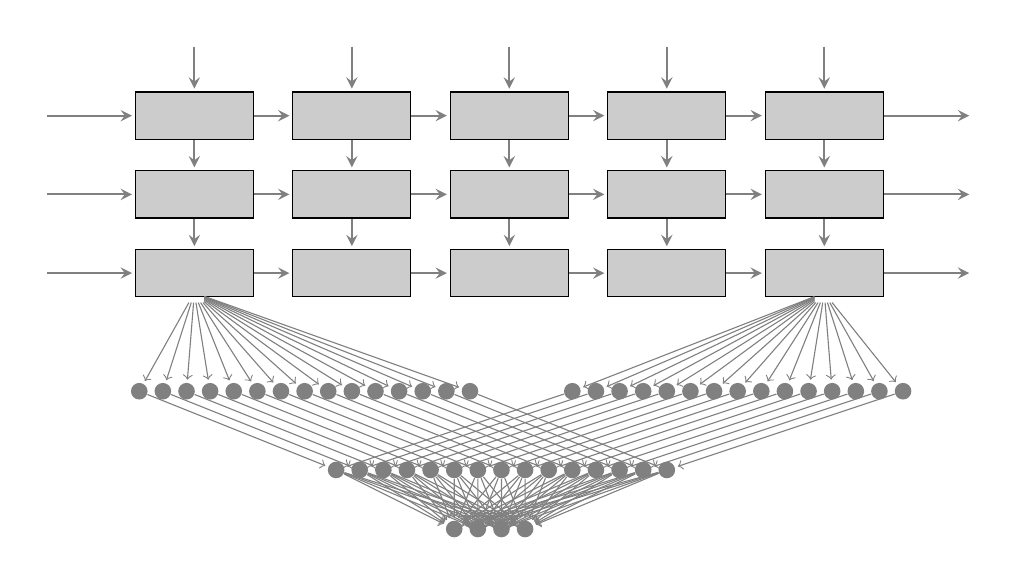
\begin{tikzpicture}[shorten >=1pt,->,draw=black!50, node distance=1cm]
      \tikzstyle{arrow} = [thick,->,>=stealth]
       \tikzstyle{every pin edge}=[<-,shorten <=1pt]
       \tikzstyle{neuron}=[circle,fill=black!50,minimum size=6pt,inner sep=0pt]

      \tikzstyle{startstop} = [rectangle, minimum width=1.5cm, minimum height=.6cm, text centered, draw=black, fill=black!20]
      \node (input) [] at (0cm,1cm) {};
      \node (output) [] at (0cm,-2.25cm) {};
      \node (s-input-A) [] at (-2cm,0cm) {};
      \node (s-output-A) [] at (10cm,0cm) {};
      \node (s-input-B) [] at (-2cm,-1cm) {};
      \node (s-output-B) [] at (10cm,-1cm) {};
      \node (s-input-C) [] at (-2cm,-2cm) {};
      \node (s-output-C) [] at (10cm,-2cm) {};
      \path[] node[startstop] (A-0) at (0cm,0cm) {};
      \path[] node[startstop] (B-0) at (0cm,-1cm) {};
      \path[] node[startstop] (C-0) at (0cm,-2cm) {};
      \draw [arrow] (input) -- (A-0);
      \draw [arrow] (s-input-A) -- (A-0);
      \draw [arrow] (s-input-B) -- (B-0);
      \draw [arrow] (s-input-C) -- (C-0);
      \draw [arrow] (A-0) -- (B-0);
      \draw [arrow] (B-0) -- (C-0);
      %\draw [arrow] (C) -- (output);

       \foreach \i/\j in {1/0,2/1,3/2,4/3}
       {
         \node (input-\i) [] at (2*\i cm,1cm) {};
         \node (output-\i) [] at (2*\i cm,-2.25cm) {};
         \path[] node[startstop] (A-\i) at (2*\i cm,0cm) {};
         \path[] node[startstop] (B-\i) at (2*\i cm,-1cm) {};
         \path[] node[startstop] (C-\i) at (2*\i cm,-2cm) {};
         \draw [arrow] (A-\i) -- (B-\i);
         \draw [arrow] (B-\i) -- (C-\i);
         \draw [arrow] (input-\i) -- (A-\i);
         \draw [arrow] (A-\j) -- (A-\i);
         \draw [arrow] (B-\j) -- (B-\i);
         \draw [arrow] (C-\j) -- (C-\i);
         %5\draw [arrow] (C-\i) -- (output-\i);
       }
       \draw [arrow] (A-4) -- (s-output-A);
       \draw [arrow] (B-4) -- (s-output-B);
       \draw [arrow] (C-4) -- (s-output-C);

       \foreach \name / \x in {1,...,15} {
           \path[xshift=-1cm]
               node[neuron] (I-\name) at (0.3*\x,-3.5cm) {};
               \path (output) edge (I-\name);
               }

       \foreach \name / \x in {1,...,15} {
           \path[xshift=4.5cm]
               node[neuron] (J-\name) at (0.3*\x,-3.5cm) {};
              \path (output-4) edge (J-\name); }

       \foreach \name / \x in {1,...,15}{
           \path[xshift=1.5cm]
               node[neuron] (K-\name) at (0.3*\x,-4.5cm) {};
          \path (I-\name) edge (K-\name);
          \path (J-\name) edge (K-\name); }

          \foreach \name / \x in {1,...,4}{
              \path[xshift=3cm] node[neuron] (O-\name) at (0.3*\x,-5.25cm) {};
              \foreach \j in {1,...,15}{
             \path (K-\j) edge (O-\name);}
             }
  \end{tikzpicture}

\end{frame}


\defverbatim[colored]\lstI{
\begin{lstlisting}[language=Python,basicstyle=\ttfamily,keywordstyle=\color{red}]
SEQ_LENGTH = 256
E_DIM = 128
STATE_DIM = 512
NUM_CLASSES = 4
def inference():
    model_input = tf.placeholder('uint8', shape=[None, SEQ_LENGTH])
    _ = tf.one_hot(Globals.model_input, depth=E_DIM, axis=-1)
    _ = tf.reshape(_, [-1, SEQ_LENGTH, E_DIM])
    fw = multi_layer_rnn(N_LAYERS, STATE_DIM)
    bw = multi_layer_rnn(N_LAYERS, STATE_DIM)
    output, _ = tf.nn.bidirectional_dynamic_rnn(fw, bw, _, dtype=tf.float32)
    fw_output = tf.reshape(output[0][:, -1:], [-1, STATE_DIM])
    bw_output = tf.reshape(output[1][:, :1], [-1, STATE_DIM])
    f = project(fw_output, E_DIM)
    b = project(bw_output, E_DIM)
    e = tf.add(f, b)
    Globals.model_output = project(e, NUM_CLASSES)
    Globals.prediction = tf.cast(tf.argmax(Globals.model_output, 1), tf.uint8)
    return Globals.model_input, Globals.model_output
\end{lstlisting}
}

\begin{frame}{A many-to-one example (code)}
\lstI
\end{frame}

\begin{frame}{A many-to-one example (output)}

\end{frame}




\begin{frame}{A many-to-many example}
\end{frame}

\begin{frame}{A many-to-many example (model architecture)}
  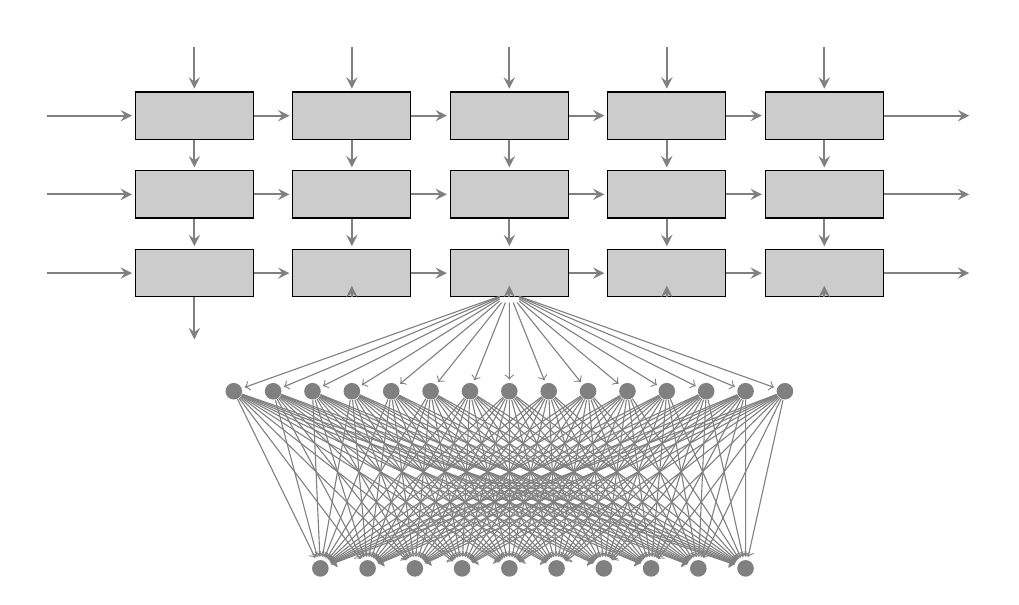
\begin{tikzpicture}[shorten >=1pt,->,draw=black!50, node distance=1cm]
      \tikzstyle{arrow} = [thick,->,>=stealth]
      \tikzstyle{startstop} = [rectangle, minimum width=1.5cm, minimum height=.6cm, text centered, draw=black, fill=black!20]
      \tikzstyle{neuron}=[circle,fill=black!50,minimum size=6pt,inner sep=0pt]

      \node (input) [] at (0cm,1cm) {};
      \node (output) [] at (0cm,-3cm) {};
      \node (s-input-A) [] at (-2cm,0cm) {};
      \node (s-output-A) [] at (10cm,0cm) {};
      \node (s-input-B) [] at (-2cm,-1cm) {};
      \node (s-output-B) [] at (10cm,-1cm) {};
      \node (s-input-C) [] at (-2cm,-2cm) {};
      \node (s-output-C) [] at (10cm,-2cm) {};
      \path[] node[startstop] (A-0) at (0cm,0cm) {};
      \path[] node[startstop] (B-0) at (0cm,-1cm) {};
      \path[] node[startstop] (C-0) at (0cm,-2cm) {};
      \draw [arrow] (input) -- (A-0);
      \draw [arrow] (s-input-A) -- (A-0);
      \draw [arrow] (s-input-B) -- (B-0);
      \draw [arrow] (s-input-C) -- (C-0);
      \draw [arrow] (A-0) -- (B-0);
      \draw [arrow] (B-0) -- (C-0);
      \draw [arrow] (C-0) -- (output);

       \foreach \i/\j in {1/0,2/1,3/2,4/3}
       {
         \node (input-\i) [] at (2*\i cm,1cm) {};
         \node (output-\i) [] at (2*\i cm,-2.25cm) {};
         \path[] node[startstop] (A-\i) at (2*\i cm,0cm) {};
         \path[] node[startstop] (B-\i) at (2*\i cm,-1cm) {};
         \path[] node[startstop] (C-\i) at (2*\i cm,-2cm) {};
         \draw [arrow] (A-\i) -- (B-\i);
         \draw [arrow] (B-\i) -- (C-\i);
         \draw [arrow] (input-\i) -- (A-\i);
         \draw [arrow] (A-\j) -- (A-\i);
         \draw [arrow] (B-\j) -- (B-\i);
         \draw [arrow] (C-\j) -- (C-\i);
         \draw [arrow] (C-\i) -- (output-\i);
       }
       \draw [arrow] (A-4) -- (s-output-A);
       \draw [arrow] (B-4) -- (s-output-B);
       \draw [arrow] (C-4) -- (s-output-C);

       \foreach \name / \x in {1,...,15}{
           \path[xshift=0cm]
               node[neuron] (K-\name) at (0.5*\x,-3.5cm) {};
          \path (output-2) edge (K-\name);
          %\path (J-\name) edge (K-\name);
          }

          \foreach \name / \x in {1,...,10}{
              \path[xshift=1cm] node[neuron] (O-\name) at (0.6*\x,-5.75cm) {};
              \foreach \j in {1,...,15}{
             \path (K-\j) edge (O-\name);}
             %\path (J-\name) edge (K-\name);
             }
  \end{tikzpicture}
\end{frame}


\defverbatim[colored]\lstI{
\begin{lstlisting}[language=Python,basicstyle=\ttfamily,keywordstyle=\color{red}]
SEQ_LENGTH = 256
E_DIM = 128
STATE_DIM = 512
N_LAYERS = 3

def inference():
    model_input = tf.placeholder('uint8', shape=[None, SEQ_LENGTH])
    _ = tf.one_hot(Globals.model_input, depth=E_DIM, axis=-1)
    encode = multi_layer_rnn(N_LAYERS, STATE_DIM)
    state_tuple = tuple(tf.unstack(Globals.initial_state, axis=0))
    output, state = tf.nn.dynamic_rnn(encode, _,
                                      dtype=tf.float32,
                                      initial_state=state_tuple)
    output = tf.reshape(output, [-1, STATE_DIM])
    output = project(output, E_DIM)
    out = tf.cast(tf.argmax(output, 1), tf.uint8)
    out = tf.reshape(out, [-1, SEQ_LENGTH])
    Globals.generated_sequence = out
    Globals.generated_characters = tf.nn.softmax(output)
    Globals.model_output = output
    Globals.state = state
\end{lstlisting}
}

\begin{frame}{A many-to-many example (code)}
\lstI
\end{frame}

\begin{frame}{A many-to-many example (output)}

\end{frame}



\defverbatim[colored]\lstI{
\begin{lstlisting}[language=Python,basicstyle=\ttfamily,keywordstyle=\color{red}]
def generate_text(length, session=None):
    generated_text = ''
    character = [[ord(' ')]]
    istate = np.zeros([N_LAYERS, 1, STATE_DIM])
    while len(generated_text) < length:
        feed_dict = {Globals.model_input: character,
                     Globals.initial_state: istate}
        next_char, state = session.run([Globals.generated_characters,
                                        Globals.state],
                                       feed_dict=feed_dict)
        next_char = np.asarray(next_char).astype('float64')
        next_char = next_char / next_char.sum()
        op = np.random.multinomial
        next_char_id = op(1, next_char.squeeze(), 1).argmax()
        next_char_id = next_char_id if chr(next_char_id) in \
                          string.printable else ord(" ")
        generated_text += chr(next_char_id)
        character = [[next_char_id]]
        istate = state
    return generated_text
\end{lstlisting}
}


\begin{frame}{A many-to-many example (text generating)}
\lstI
\end{frame}

 \begin{frame}{Many-to-one-to-many example}

\begin{itemize}
\item  A recurrent neural network that can sort sequences
\item Two parts: an encoder, and a decoder
\item The encoder encodes sequences into fixed length vectors
\item The decoder transforms this vector into a sorted list of numbers.
\end{itemize}

 \end{frame}



 \begin{frame}{Many-to-one-to-many example}

   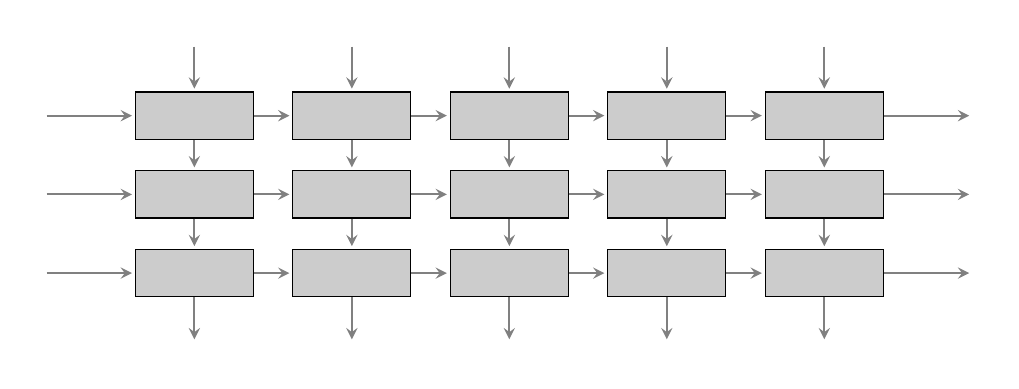
\begin{tikzpicture}[shorten >=1pt,->,draw=black!50, node distance=1cm]
       \tikzstyle{arrow} = [thick,->,>=stealth]
       \tikzstyle{startstop} = [rectangle, minimum width=1.5cm, minimum height=.6cm, text centered, draw=black, fill=black!20]
       \node (input) [] at (0cm,1cm) {};
       \node (output) [] at (0cm,-3cm) {};
       \node (s-input-A) [] at (-2cm,0cm) {};
       \node (s-output-A) [] at (10cm,0cm) {};
       \node (s-input-B) [] at (-2cm,-1cm) {};
       \node (s-output-B) [] at (10cm,-1cm) {};
       \node (s-input-C) [] at (-2cm,-2cm) {};
       \node (s-output-C) [] at (10cm,-2cm) {};
       \path[] node[startstop] (A-0) at (0cm,0cm) {};
       \path[] node[startstop] (B-0) at (0cm,-1cm) {};
       \path[] node[startstop] (C-0) at (0cm,-2cm) {};
       \draw [arrow] (input) -- (A-0);
       \draw [arrow] (s-input-A) -- (A-0);
       \draw [arrow] (s-input-B) -- (B-0);
       \draw [arrow] (s-input-C) -- (C-0);
       \draw [arrow] (A-0) -- (B-0);
       \draw [arrow] (B-0) -- (C-0);
       \draw [arrow] (C-0) -- (output);

        \foreach \i/\j in {1/0,2/1,3/2,4/3}
        {
          \node (input-\i) [] at (2*\i cm,1cm) {};
          \node (output-\i) [] at (2*\i cm,-3cm) {};
          \path[] node[startstop] (A-\i) at (2*\i cm,0cm) {};
          \path[] node[startstop] (B-\i) at (2*\i cm,-1cm) {};
          \path[] node[startstop] (C-\i) at (2*\i cm,-2cm) {};
          \draw [arrow] (A-\i) -- (B-\i);
          \draw [arrow] (B-\i) -- (C-\i);
          \draw [arrow] (input-\i) -- (A-\i);
          \draw [arrow] (A-\j) -- (A-\i);
          \draw [arrow] (B-\j) -- (B-\i);
          \draw [arrow] (C-\j) -- (C-\i);
          \draw [arrow] (C-\i) -- (output-\i);
        }
        \draw [arrow] (A-4) -- (s-output-A);
        \draw [arrow] (B-4) -- (s-output-B);
        \draw [arrow] (C-4) -- (s-output-C);

   \end{tikzpicture}
 \end{frame}


 \defverbatim[colored]\lstI{
 \begin{lstlisting}[language=Python,basicstyle=\ttfamily,keywordstyle=\color{red}]
   SEQ_LENGTH = 256
   E_DIM = 128
   STATE_DIM = 512
   N_LAYERS = 4

   def inference():
       model_input = tf.placeholder('uint8',
                                    shape=[None, SEQ_LENGTH])
       _ = tf.one_hot(model_input, depth=E_DIM, axis=-1)
       _ = tf.reshape(_, [-1, SEQ_LENGTH, E_DIM])
       encode = multi_layer_rnn(N_LAYERS, STATE_DIM)
       OP = tf.nn.dynamic_rnn
       encoded_input, state = OP(encode,_,dtype=tf.float32)
       Globals.encoder_output = state
       with tf.variable_scope('decoder'):
           training_decoder_input = tf.zeros_like(Globals.model_input)
           _ = tf.one_hot(training_decoder_input, depth=E_DIM, axis=-1)
           _ = tf.reshape(_, [-1, SEQ_LENGTH, E_DIM])
           decode = multi_layer_rnn(N_LAYERS, STATE_DIM)
           decoded_output, state = tf.nn.dynamic_rnn(decode, _,
                                                     dtype=tf.float32,
                                                     initial_state=state)
           decoded_output = tf.reshape(decoded_output, [-1, STATE_DIM])
           output = project(decoded_output, E_DIM)
           out = tf.cast(tf.argmax(output, 1), tf.uint8)
           out = tf.reshape(out, [-1, SEQ_LENGTH])
           Globals.training_decoder_input = training_decoder_input
           Globals.model_output = output
           Globals.prediction = out
           Globals.decoder = decode
           Globals.decoder_input = _
 \end{lstlisting}
 }
 \begin{frame}{Many-to-one-to-many example code}
   \lstI
 \end{frame}


 \begin{frame}{A many-to-one-to-many example (output)}
 \end{frame}

 \begin{frame}{A many-to-one-to-many example (output)}
 \end{frame}

 \begin{frame}{A many-to-one-to-many example (output)}
 \end{frame}

 \begin{frame}{A many-to-one-to-many example (output)}
 \end{frame}

 \begin{frame}{A many-to-one-to-many example (output)}
 \end{frame}

 \begin{frame}{A many-to-one-to-many example (output)}
 \end{frame}


\end{document}
